%
\chapter{Introduction}\label{chap:introduction}%
%
    \textit{%
        In light of the depletion of conventional, natural and fossil fuels for energy production, as well as their negative impact of their consumption on the environment, renewable, clean - virtually emissionless - and readily available alternatives are direly called for. Despite its, for now more than 70 years persisting technical and economical challenges, magnetically confined plasma nuclear fusion is a prime candidate for such and has the potential to be the final answer to issues of ongoing climate change, the associated accelerated growth in energy consumption, costs and the discrepancy of global resource distribution\cite{IPCC2023,Toschi1971}.
    }%
%
    \section{Nuclear Fusion}\label{sec:section}%
%
        Nuclear fusion is the process of two lighter atoms or nuclei interacting and forming a heavier element. This phenomenon has been thoroughly studied since its discovery in the early 20th century on our solar systems central star \textit{sol}\cite{Oliphant1934}. Ironically, initial research around nuclear fusion was based on weapons development surrounding the \textit{Manhattan Project}\footnote[1]{a program of research and development during WWII to produce nuclear weapons, led by the United States in collaboration with the United Kingdom, resulting in two bombs dropped on Japan} \textit{thermonuclear bombs} and later iterated upon by scientist in the United Kingdom and finally brought to a first concept individually in 1950/51 by Lyman Spitzer\footnote[2]{Lyman Spitzer, Jr. *\,Jun. 26, 1914 Toledo; \textdagger\,Mar. 31, 1997 Princeton} in the USA, as well as Andrei Sacharow\footnote[3]{Andréj Dmítrievič Sácharov, *\,May 21, 1921 Moscow; \textdagger\,Dec. 14, 1989} and Igor Tamm\footnote[4]{Igor' Evgen'evič Tamm, *\,Jun. 26, 1895 Wladiwostok; \textdagger\, Apr. 12, 1971 Moscow} in the USSR. All postulated magnetic plasma confinement as way to a thermonuclear reactor, however with different approaches, i.e. the \textit{stellarator} and \textit{tokamak}. Since then, nuclear fusion has been experimentally demonstrated in laboratory environments and hence associated with the fourth state of matter, \textit{plasma}\cite{Shafranov2001}.\\%
        Fusion processes involving light nuclei, i.e. hydrogen or helium isotopes are energetically most advantageous, as they produce the most energy per nucleus mass. In the case of confined, high-temperature plasma applications, such large kinetic energies and therefore velocities are necessary to overcome the electrostatic Coulomb force repulsion between the positively charged nuclei, reducing the distance so that the \textit{strong nuclear force} dominates, and fusion reactions are induced. Rate coefficients $\left\langle\sigma v\right\rangle$ towards the total yield $Q=P\ix{fus}/P\ix{ext}$, with $P\ix{fus}$ the power from fusion reactions and $P\ix{ext}$ the input, are convolutions of kinematic cross-sections and Maxwell-Boltzmann distributions. Of those, only a Deuterium-Tritium interaction has a large enough contribution at energies $\le$\SI{64}{\kilo\electronvolt} due to an intermittent resonance in a volatile $^{5}_{2}$He\cite{Bosch1992}.
%
            \begin{align}%
                ^{2}_{1}\text{D}+\,^{3}_{1}\text{T}\longrightarrow\,^{5}_{2}\text{He}^{\ast}\longrightarrow\,^{4}_{2}\text{He}\left(\text{\SI{3.5}{\mega\electronvolt}}\right)+\,^{1}_{0}n\left(\text{\SI{14.1}{\mega\electronvolt}}\right)\label{eq:dtfus}%
            \end{align}%
%
        Resulting kinetic energies of the products are noted accordingly. Plasma temperatures of \SI{20}{\kilo\electronvolt} have been achieved regularly and by a large range of devices, underlining the superiority of DT fusion in this regard. The vast energy gain on the right-hand-side in \cref{eq:dtfus}, particularly the fast neutrons can be used to heat a water repository in a future power plant, similar to a conventional nuclear fission reactor. Additionally, only minor secondary radioactive waste from neutron activation is expected from such a device, alleviating the issue of dismantlement and final storage of other nuclear machines. Deuterium has a sufficient natural abundance and hence can be distilled effectively from water, while Tritium does not but can be \textit{bred} using the penetrating neutrons and a supplementary Lithium blanket around the vessel.\\%
%
        \newline%
        This thesis is concerned with the properties of radiation in the stellarator \textit{Wendelstein-7X} (W7-X), particularly from intrinsic and extrinsic impurities, their transport and effects on the overall plasma performance. After an introduction to the machine, presented results will be centred around the core diagnostic responsible for measuring radiation at W7-X: the \textit{multicamera, metal resistor bolometer}. The next sections will introduce the core concepts relating to the investigations performed in this work.%
%
    \section{Wendelstein 7-X}\label{sec:w7x}%
%
        \begin{figure}%
            \centering%
            \includegraphics[width=0.5\textwidth]{%
                content/figures/chapter0/w7x}%
            \caption{Stellarator Wendelstein 7-X: Cut-away rendering of the outer vessel, superconducting magnetic coils, cooling and supporting structure. The plasma (last close flux surface, \textcolor{pink}{pink}) located in a vacuum vessel, confined by non-planar coils (\textcolor{gray}{gray}) and adjusted through planar coils (\textcolor{orange}{orange}), e.g. to radially position the plasma. Magnetic superstructure and inner containment vessel are surrounded by the cryostat (\textcolor{gray}{gray}). \textcopyright IPP}\label{fig:w7x}%
        \end{figure}%
%
        Wendelstein 7-X is the latest iteration in a long line of stellarator experiments conducted by scientists at the Max-Planck Institute for Plasma Physics, beginning in the 1950s. The first W1-A stellarator went into operation in 1960 at the Max-Planck Institute for Physics and Astrophysics, providing a foundation for the continuing development of which this device is the culmination.\\%
        Stellarators generate the necessary rotational transform, the twist of the magnetic field, (majorly) by external coils. A purely toroidal field is not sufficient to confine a quasineutral plasma: the magnetic curvature and field gradient lead to a charge separated drift in opposite directions, resulting in a vertical electric field and conclusively to an outward $\vec{E}\times\vec{B}$ motion. Consequently, the stellarator magnetic field is deliberately configured using said coils to achieve helicity and an essentially current-less plasma that is more stable compared to a tokamak. Wendelstein 7-X is designed to be modular, i.e. have a discrete symmetry that enables entire subsections to be replaced or exchanged. The iterative optimisation process towards such a modular device was shaped to satisfy multiple criteria, including small magnetic islands, good plasma equilibrium and magnetohydrodynamic (MHD) stability, reduced neoclassical transport, minimized bootstrap current and fast particle confinement. Its modular designed, five-fold symmetric superconducting magnetic field coils encompass the whole machine. The coil system consists of 70 superconducting magnets of seven different shapes, 50 non-planar coils producing the twisted magnetic field and 20 planar coils for increased flexibility in magnetic configuration space - it can be seen in \cref{fig:w7x}\cite{Spitzer1958,Boozer1998,Wagner1998,Beidler1990}.\\%
        The W7-X stellarator is the largest of its kind, with a major and minor radius of \SI{5.5}{\meter} and \SI{0.53}{\meter} (depending on magnetic coil currents) respectively, volume of \SI{30}{\cubic\meter}, \SI{3}{\tesla} maximum magnetic field strength, heating power of \SI{14}{\mega\watt} and expected plasma temperatures of up to \SI{130}{\mega\kelvin}. W7-X has performed three successful experimental campaigns since its first plasma in 2015. After multiple upgrades, the machine has demonstrated improved, longer confinement and increased overall power, with the ultimate goal being a discharge duration of \SI{30}{\minute} at \SI{10}{\mega\watt} of external heating, demonstrating a capability essential to a future fusion power plant: continuous operation\cite{Klinger2016_2}.\\%
        Development of this stellarator reactor line was defined by the qualification of a viable divertor concept. Divertors - interfaces deliberately contacting and \textit{diverting} (interacting) with the hot plasma - in stellarators cannot be toroidally symmetric. The cross-section of W7-X varies strongly from triangular to bean-shaped and exhibits natural magnetic islands. Wendelstein 7-X features magnetic configurations with five field periods, each being stellarator symmetric (flip symmetric). There are two up/down-symmetric toroidal planes in each period, 36$^{\circ}$ degrees apart toroidally and containing both bean-shaped and triangular cross-sections. So-called \textit{island divertors} are placed at the edge where the rotational transform $\iota$ has a resonance close to unity - number of poloidal transits per single toroidal transit of a field line on a toroidal flux surface -, i.e. where these islands are located. The tube of the last closed flux surface (LCFS) and cuts through the magnetic field structure for characteristic points can be found in \cref{fig:trianglebeanFS}. On each magnetic field period, one pair of island divertor modules is installed where the cross-section of the magnetic field is predominately bean-shaped. Magnetic islands intersect these targets, providing a well-defined flow of particles from the plasma \textit{scrape-off layer} (SOL) to the wall and decoupling the core plasma region in the process. Divertors therefore have to withstand a heat flux of up to \SI{10}{\mega\watt\per\square\meter}.  
        The W7-x island divertor can operate at $-\iota=5/6$,\,5/5 (standard divertor configuration) and 5/4 resonances. Standard configuration can be achieved using only non-planar coils, with \textit{high-} and \textit{low-}$\iota$ also applying planar coils. Both radial island width and connection length along field lines to the islands can be manipulated with the magnetic configuration, impacting e.g. transport end exhaust of impurities. A more detailed description of the magnetic configuration space can be found in \cite{Geiger2015}. Wendelstein 7-X was not yet equipped with water-cooling and plasma contact points are only inertially cooled in experiments discussed for this thesis\cite{Geiger2015,Beidler1990}.%
%
        \begin{figure}%
            \centering%
            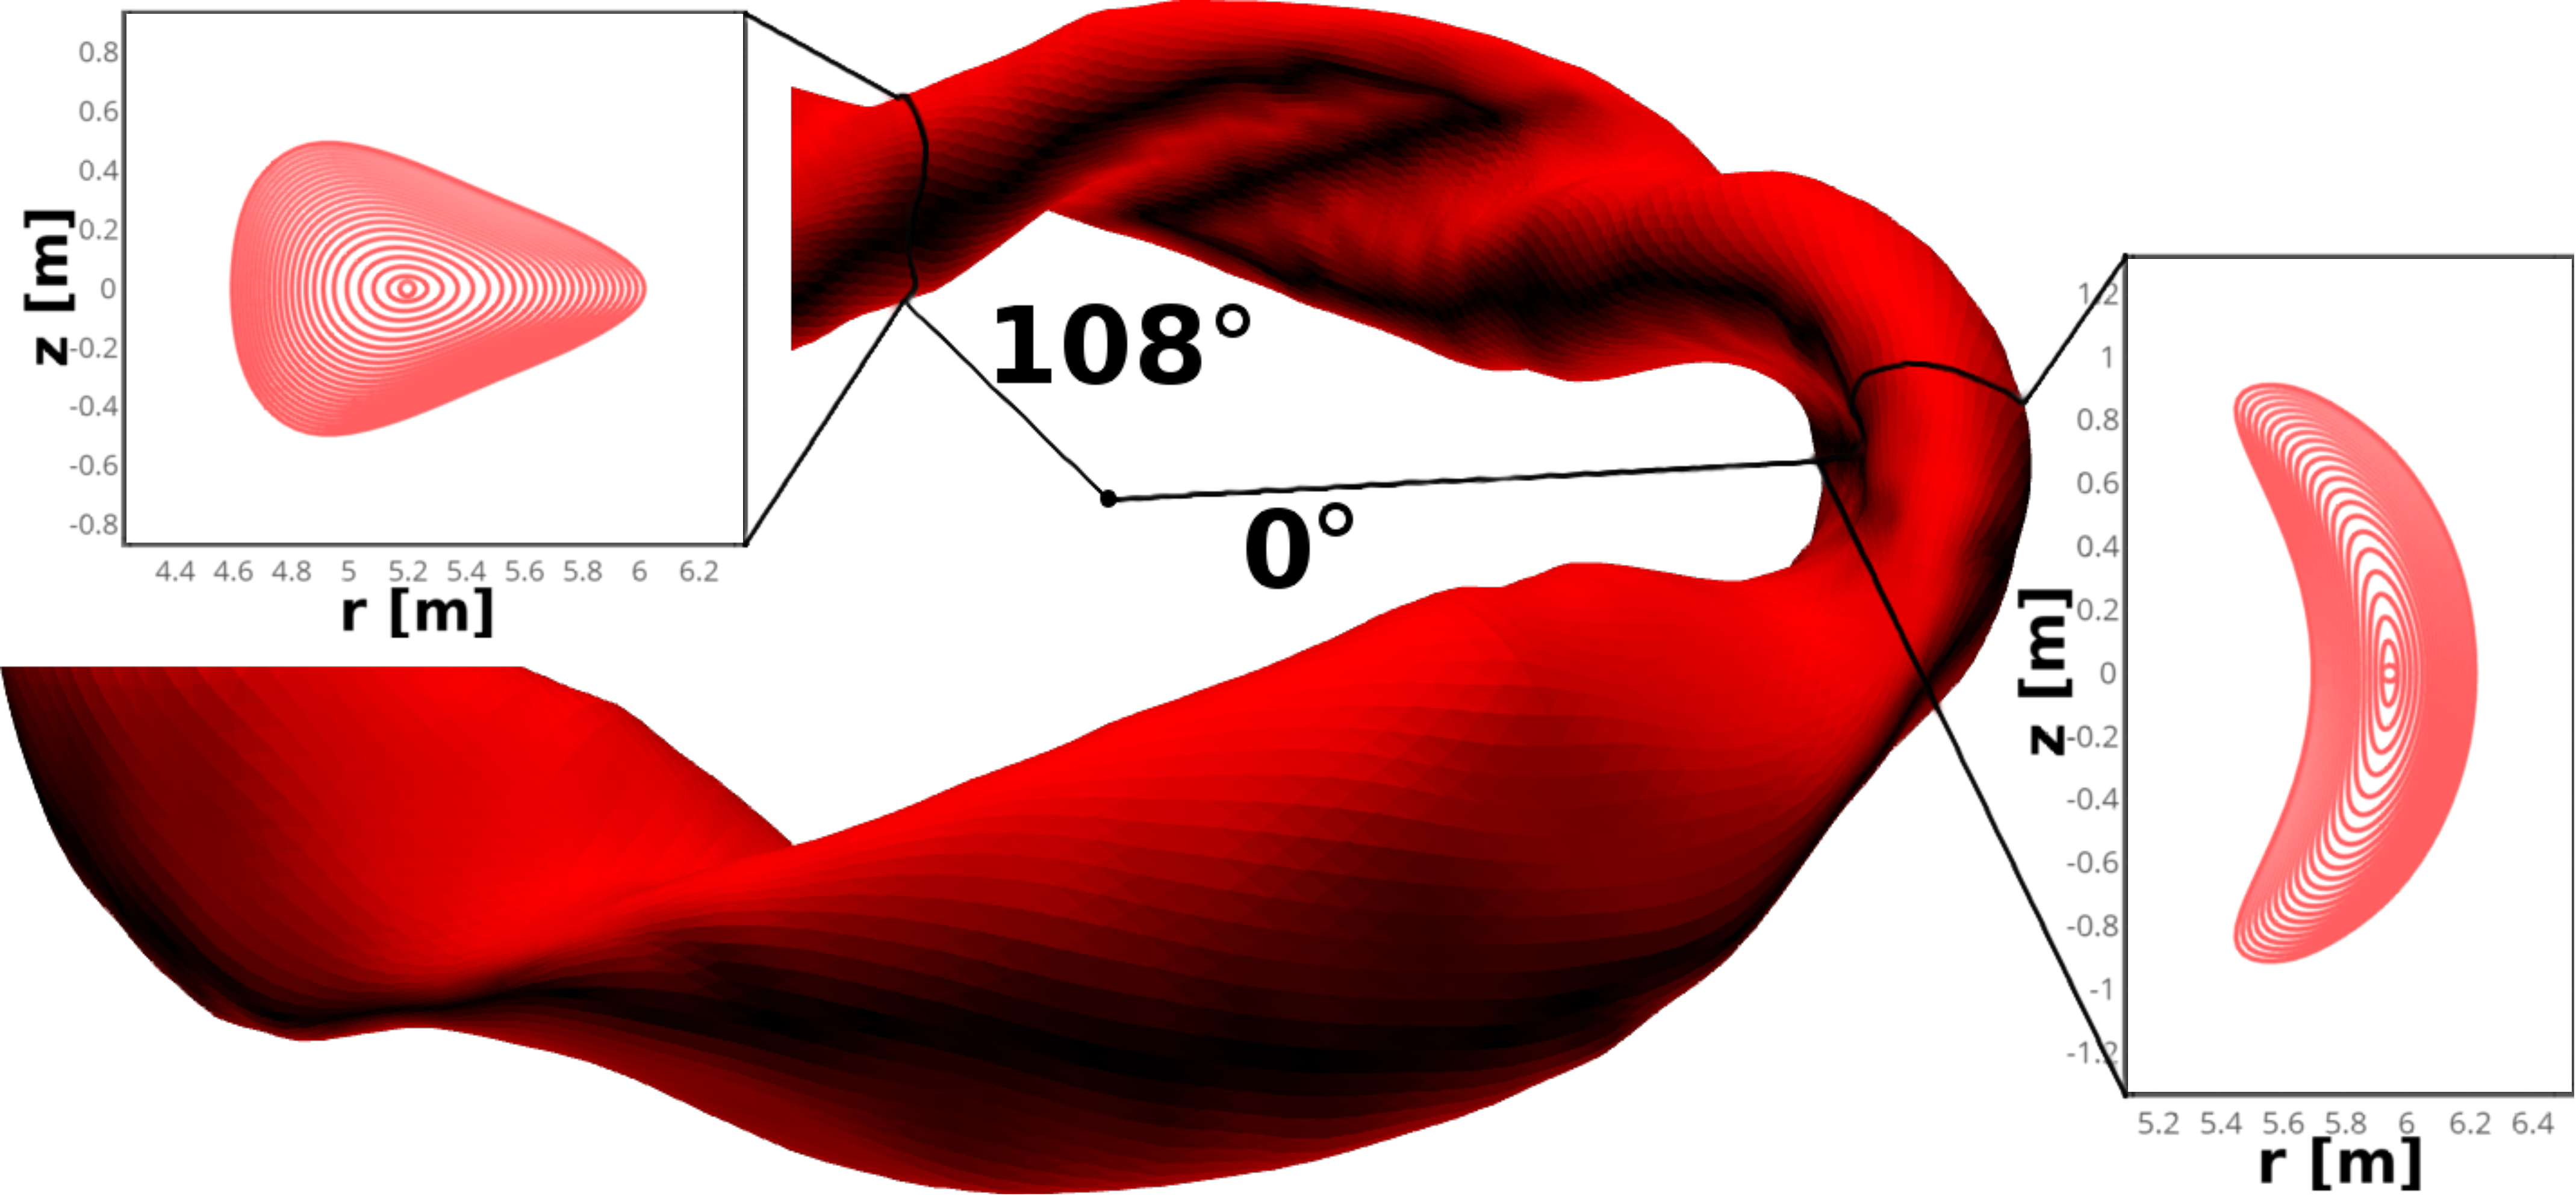
\includegraphics[width=0.6\textwidth]{%
                content/figures/chapter0/torus_full_banana_alpha.png}%
            \caption{Flux tube of the last closed flux surface around the W7-X torus and cross-sections in the triangle- (left) and bean-shaped (right)plane. At \SI{108}{\degree} toroidally, the bolometer camera system is located.}\label{fig:trianglebeanFS}%
        \end{figure}%
%
    \section{Plasma Physics}\label{sec:plasmaphysics}%
%
        At the given temperatures, matter only exists as plasma, an ionized gas where atoms are fully ionized and interact with electric and magnetic fields. Hence, fusion energy research is the study of high-temperature plasma physics in large devices with strong magnets. Challenges here are the long-time confinement of particles and exhaust of thermal energy, while a lower limit for a self-sustaining or -heating fusion plasma $Q>1$ - the fusion energy gain factor is the ratio of fusion power produced in a nuclear fusion reactor to the power required to maintain the plasma in steady state - is given by the \textit{triple product} or \textit{Lawson\footnote[1]{John David Lawson FRS; * Apr 4, 1923; \textdagger Jan 15, 2008 - British engineer and physicist} criterion}. Originally it was derived from the concept that the total net power in excess is equal to the energy produced by fusion itself, minus radiative and kinetic losses under the  assumption of an intrinsic efficiency of the machine, as it would the case for any conventional power plant. Introducing an energy confinement time $\tau\ix{E}$, measuring the rate at which a unit of energy is lost from the plasma to its enclosing system, and making further assumptions about the energy distribution of particles species, this can be written into the \textit{triple product} $n\ix{e}T\tau\ix{E}$. Non-hydrogenic species in the plasma from deliberate gas puffing, solid-state seeding, sputtering of wall material or intrinsic impurities have to be taken into account due to their parasitic and diluting - decreasing the likelihood of two hydrogen particles interacting - effect on the system as well:%
%
        \begin{align}%
            n\ix{e}T\tau\ix{E}\ge\frac{12f\ix{tot}}{\left\langle\sigma\ix{DT}v\right\rangle f\ix{H}^{2}E_{\alpha}-4L\ix{Z}\left(T\right)}\,T^{2}\,\,\label{eq:lawson}%
        \end{align}%
%
        with $n\ix{x}$ the number densities and $T$ the equilibrated temperatures of electrons, ions and atomic hydrogen respectively, $f\ix{H}=n\ix{H}/n\ix{e}$ the hydrogens' dilution, $f\ix{tot}=\sum_{i}n\ix{i}/n\ix{e}$ the ion-electron dilution, $E_{\alpha}$ kinetic alpha particle energy and $L\ix{Z}$ the radiative loss function. Plasma conditions described by satisfying the Lawson criterion in \cref{eq:lawson} require a strong confinement. On stellar scales, gravitation can provide the needed entrapment of particles, i.e. in objects with sufficient mass like \textit{red dwarfs}. Experiments have also used inertial confinement, exploding pellets of fuel and using the high temperature and density on the inside upon implosion to achieve fusion reactions. In the context of large scale reactors, strong magnetic fields trap charged particles by Lorentz force to restrict their motion perpendicular to its field, travelling in a \textit{gyro-motion} on helical trajectories along those lines. \cite{Helander2014,Boozer2015}.\\%
        In current and future plasma fusion devices, large heat loads on plasma facing components are a challenge and topics surrounding it of great scientific interest, as steady-state operation at large powers is central to the ultimate goal of a nuclear fusion power plant. The expected huge power flux onto divertors for such a scenario of continuous operation are significantly larger than the material limits. Distribution of this energy and thermal load through electromagnetic radiation into the full $4\pi$ solid angle and onto the entire vessel wall is one possible solution to this problem. \textit{Bremsstrahlung} $P\ix{brems}$ of accelerating charged particles on field lines and line radiation from ionisation and excitation processes $P\ix{line}$ contribute to the \textit{cooling} of the core. Steady-state, the plasma confinement power balance can be written as $P_{\alpha}+P\ix{h}=P\ix{n}+P\ix{rad}^{\text{core}}+P\ix{SOL}$, with $P_{\alpha}$ the alpha particle energy, $P\ix{n}$ the neutron energy, $P\ix{h}$ the external input, $P\ix{SOL}$ the total power in the SOL and $P\ix{rad}^{\text{core}}=P\ix{brems}+P\ix{line}$. Introduction or seeding of extrinsic, high-Z impurities into the core, which radiate strongest in the hotter confinement center can be used to increase the latter and hence reduce the power that enters the SOL\cite{Shubov2021,Schneider2006,Drawin1978}. The impact of deliberate plasma pollution however has drawbacks. Dilution is increased because of their higher charge and are likely to accumulate in the core due to transport dynamics. Furthermore, oversaturation with impurities can lead to plasma termination or radiative collapses. Varying operational and machine conditions, as well as impurity species inside the plasma and their different behaviour under those circumstances make the experimental evaluation particularly difficult\cite{Reimold2015}. This topic is center of ongoing investigations and ultimately motivation for the methodology and application developed over the course of this thesis. In the hypothetical first plasma fusion power plant prototype DEMO, it is expected that $0.7P\ix{$\alpha$H}$ - the alpha particles plasma heating power - is radiatively exhausted from the core and the remainder has to be further reduced through radiation in the SOL, finding at least a radiation fraction $f\ix{rad}=P\ix{rad}/P\ix{$\alpha$H}>0.95$. \textit{Radiation in the divertor} has several benefits, like decreased physical sputtering of wall material and additional reaction loss channels with neutral particles, reduced total heat flux onto and broadening of the contact area with the target. The latter is a result of the density increase closer to the target due to energy loss in paralell direction, which in turn again increases radiation. For lower temperatures outside the LCFS, low-Z impurities can be used to control the radiation here such that fuel dilution, impurity retention and radiative saturation of the divertor are of adequate levels\cite{Eich2013,Eich2011,Fuchert2020}.%
%
        \subsection{Transport}\label{subsec:tranport}%
%
            Transport plays a very important role in fusion devices, transferring energy, mass and charge spatially via collisions between particles, thermodynamically equilibrating the plasma. Commonly, plasma transport refers to the combination of classical, neoclassical and anomalous or turbulent processes. Turbulence very effectively transports energy and mass through the plasma, itself being generated by instabilities.%
%
            \subsubsection*{Classical Transport}%
%
                The term \textit{classical} considers \textit{Coulomb}-collisions between charged particles, causing diffusive and convective transport and eventually leading to a net particle loss from the confinement to the SOL and vessel walls. Such collisions change the center of the particles gyrating motion, with displacements the size the Larmor radius $r\ix{L}$. Same species Coulomb collisions yield no net transport but may contribute to energy transfer and heat flux. Ion-impurity collisions dominate the impurity transport due the large collision frequency $\nu$ (collisionality). The particle displacement is characterised by a diffusive $D$ and convective $v$ transport coefficient, of which the prior is orders of magnitude higher along the magnetic field lines than perpendicular. Classial transport is the fastest on a given flux surface compared to other forms of transport in equilibrating plasma species distributions. The rate of diffusion scales with $\propto1/B^{2}$, implying that confinement times can be greatly improved with small increases in field strength.\cite{Chen1984}.
%
            \subsubsection*{Neoclassical Transport}%
%
                Perpendicular transport rates suggested by classical diffusion have not been found in practice, where previously unknown plasma instabilities cause the particles to leave confinement at rates closer to $\propto B$. \textit{Neoclassical transport} provides a model for the transport of particles, momentum, and heat due to Coulomb collisions in magnetically confined plasmas. The classical model has to be extended by the incorporation of geometrical effects, which lead to complex particle orbits and drifts that were ignored in the latter.\\
                In toroidal geometries, additional drift effects greatly increase the typical particle displacement perpendicular to the magnetic field across field lines. This is called neoclassical transport and is always present in toroidal machines. Writing the Boltzmann equation with the particle distribution function $f\ix{x}=f\ix{x}\left(\vec{x},\vec{v},t\right)$ for particle species $x$, the \textit{Fokker-Planck}\footnote[1]{Adriaan Daniël Fokker; * Aug 17, 1887 Buitenzorg; \textdagger Sep. 24 1972 Beekbergen} expression for a collisionality operator and an additional source term $S\ix{x}$ gives a kinetic equation for neoclassical transport from which the respective moments can be derived\cite{WikiFokkerPlanck}.%
%
                \begin{align}%
                    \frac{\partial f\ix{x}}{\partial t}+\vec{v}\,\nabla f\ix{x}&+\frac{Z\ix{x}e}{m\ix{x}}\left(\vec{E}+\vec{v}\times\vec{B}\right)\nabla\ix{v}f\ix{x}=\nonumber\\%
                    &-\frac{\partial}{\partial v\ix{i}}\left(f\ix{x}\left\langle\Delta v\ix{i}\right\rangle\right)+\frac{1}{2}\frac{\partial^{2}}{\partial v\ix{i}\partial v\ix{j}}\left(f\ix{x}\left\langle\Delta v\ix{i}\Delta v\ix{j}\right\rangle\right)+S\ix{x}\label{eq:neoclassical}%
                \end{align}%
%
                In a collisionless regime, this reduces to the \textit{Vlasov equation}, describing temporal evolution of $f\ix{x}$ for plasma of charged particles only coupled by long-range interaction such as Coulomb interaction\cite{WikiVlasov}. Equation \ref{eq:neoclassical} satisfies momentum, particle and energy conservation and assumes that collisions only have small random effects on the particle velocity and are sufficiently frequent for the resulting particle trajectory to be described also as random, i.e. are diffusive in velocity space.\\%
                Neoclassical transport theory provides a set of equations for the temporal evolution of a species moments. It accounts for all particle motion associated with toroidal geometry, specifically $\nabla B$ and curvature drifts, passing and trapped particles, e.g. on \textit{banana orbits}. The theory is valid for all collisionality regimes, and includes effects due to resistivity and viscosity.\cite{Houlberg1997,Tribaldos2005,Fulop2001}.\\%
                In a neoclassical fluid picture, diamagnetic flows drive parallel flows. Similarly to classical transport, convection also may be written with the diamagnetic drift and the related friction between particles entering into the resulting drift velocity. Hence, a neoclassical radial flux for impurity of charge $q$ for the types of transport orbits $O=\left\{\right.$banana,\,plateau,\,Pfirsch-Schlüter$\left.\right\}$ is given by:
%
                \begin{align}%
                    \vec{\Gamma}\ix{q}=\sum^{O}_{x}\,D\ix{x}\left(-\nabla n\ix{q}+n\ix{q}q\left[\frac{\nabla n}{n}-H\ix{x}\frac{\nabla T}{T}\right]\right)=-D\ix{neo}\nabla n\ix{q}+v\ix{neo}n\ix{q}\,\,.\nonumber%
                \end{align}%
%
                In any case, the convection is proportional to the charge of the impurity and its contribution consists of one term into the direction of the density gradient and one opposite the direction of the temperature gradient depending on the parameter $H\ix{x}$, the weight factor of the normalised temperature gradient. The latter is given through plasma parameters, geometry, and the mass ratio between collision partners. For similarly oriented temperature and density gradients, $H\ix{x}$ is positive and an effect of temperature screening is observed. Convection here is proportional to the charge of the impurity, such that effects due to the neoclassical drifts are enhanced for higher charge states. Realistically, multiple impurity species lead to a critical friction equilibrium between them towards their transport fluxes\cite{Dux2000,Dux2004}.\\%
%
                \begin{figure}%
                    \centering%
                    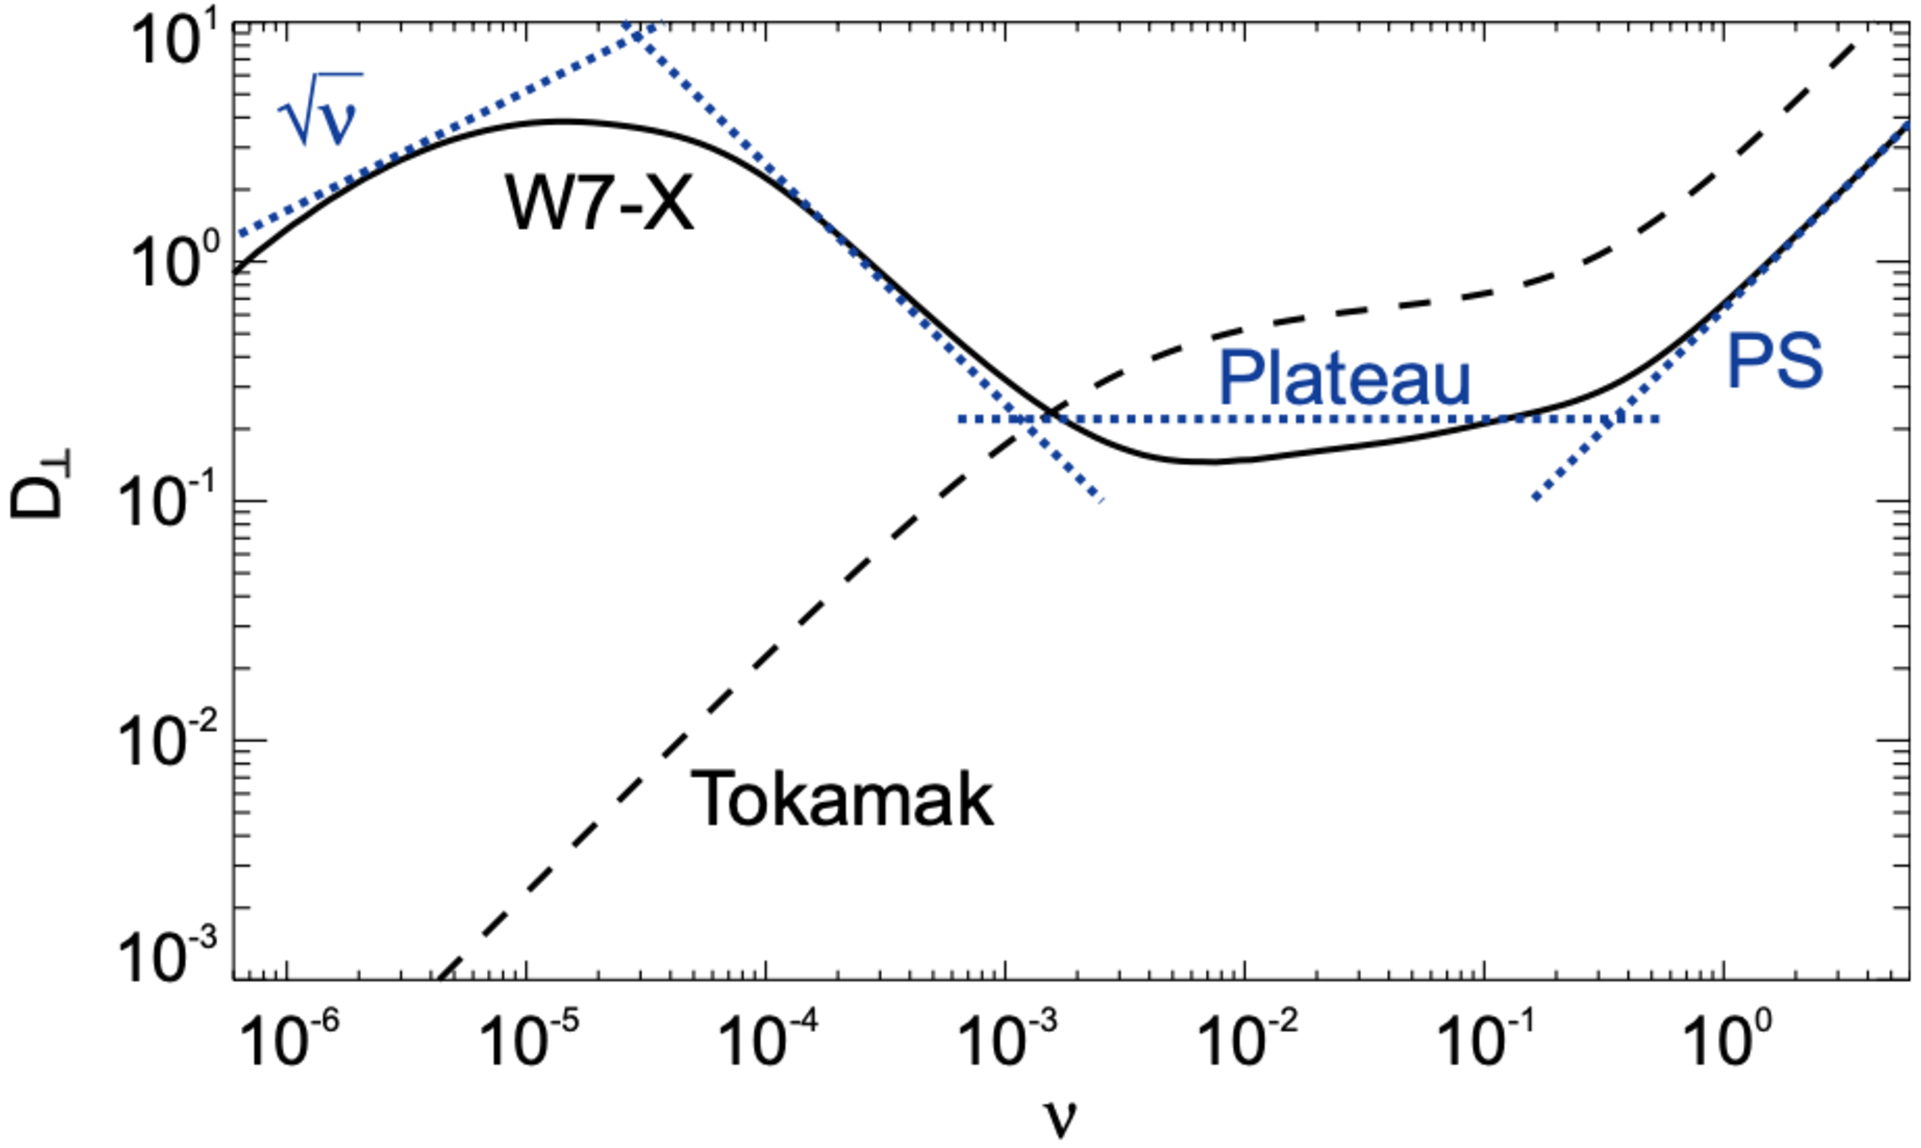
\includegraphics[width=0.5\textwidth]{%
                        content/figures/chapter0/transportRegimes.pdf}%
                    \caption{Neoclassical transport fluxes for different orbits, with the banana orbit dominating at low collisionality.\cite{Helander2012}}\label{fig:neoclassical_transport}%
                \end{figure}%
%
                Diffusive behaviour and hence the transport regimes change with collisionality, see seen \cref{fig:neoclassical_transport}. The radial or perpendicular diffusion coefficient $D_{\perp}$ describes how strong the transport is. For low collisionality, and thus larger mean free paths than the size of the device, particles become trapped on flux surfaces as they orbit multiple times before colliding. Their perpendicular kinetic energy can be neglected (\textit{banana regime/orbits}). Neoclassical diffusion strongly depends on the magnetic structure of the device, i.e. in stellarators particles may leave trapped orbits without collisions due to the fields broken symmetry, resulting in a net neoclassical transport one to two orders of magnitude higher than in tokamaks. The field geometry of W7-X was optimised to also reduce neoclassical transport in scenarios of low collisionality, decreasing perpendicular particle and energy losses. In trapped particle regimes with low collisionality, if the radial electron and ion fluxes are not equal, a resulting radial electric further shifts the balance towards ambipolarity and decoupling of the species. With electron cyclotron resonance heating (ECRH), this leads to $T\ix{e}\gg T\ix{i}$, which is highly unfavourable for fusion plasma. This decrease electron mobility also reduces neoclassical transport and is called \textit{electron-root} regime ($\propto \sqrt{\nu}$). Similarly, for higher collisionality the direction of the electric field is reversed, leading to an \textit{ion-root} regime ($\propto 1/\nu$). At even higher $\nu$, mean free paths decrease and perpendicular diffusion increases, so that particles may not complete their orbits anymore and the field geometry becomes irrelevant. This \textit{Pfirsch-Schlüter} regime is directly dependend on the classical transport $D\ix{PS}\propto D\ix{classical}$\cite{Helander2012,Helander2014}.%
%
            \subsubsection*{Anomalous Transport}%
%
                Research finds that transport exceeds neoclassical expectations by an order of magnitude or more. Differences between measurement and prediction are called \textit{anomalous} transport, generally assumed to be generated by non-linear, turbulent effects driven by micro-instabilities. An important argument for turbulence significantly contributing to the total transport to this degree is its scaling with heating power and machine size. In contradiction to neo-/classical predictive scaling laws, confinement decreases with temperature, potentially explained by greater turbulence and transport at higher $T$. Decreased energy confinement time for a given plasma size also inevitably means increasing the size of a reactor in order to meet the required triple product condition, see \cref{eq:lawson}. Furthermore, deliberate suppression of turbulent effects, either actively or passively, sees a reduction in transport, supporting the previous assumption. The general assumption is that anomalous transport is the consequence of microscopic instabilities, caused by steep density, temperature, and pressure gradients, e.g. ion and electron temperature gradient instabilities (ITG, ETG). Their spatial and temporal scales are very small, i.e. below centimenter and milliseconds, making them hard to detect and measure. Perpendicular anomalous transport is usually much larger than either neo-/classical and therefore the dominant effect in radial transport.\cite{Balescu2005,Milligen2004}.\\%
                As was highlighted before, impurities play a key role in the behaviour and performance of fusion plasma. Hence their transport is as important for understanding phenomena that are subject of this thesis. An integrated impurity flux for species $q$ can simply be written as the sum of all previous phenomena:%
%
                \begin{align}%
                    \vec{\Gamma}\ix{q}=-\left(D\ix{neo,q}+D\ix{an,q}\right)\nabla n\ix{q}+\left(v\ix{neo,q}+v\ix{an,q}\right)n\ix{q}=-D\ix{q}\nabla n\ix{q}+v\ix{q}n\ix{q}\,\,.\nonumber%
                \end{align}%
%
                Usually, dominant turbulent transport $D\ix{neo}\ll D\ix{an}$ so that neoclassical diffusion may be neglected. Only When turbulent transport is suppressed or small, neoclassical diffusion becomes important. For high charge $q$ or high-Z impurities, charge dependent terms increase the neoclassical convection so that it is noticeable outside those cases.\cite{Garcia2006,Langenberg2019}.%
%
        \subsection{Plasma Radiation}\label{subsec:radiation}%
%
            \begin{figure}[t]%
                \centering%
                \includegraphics[width=.5\textwidth]{%
                    content/figures/chapter0/%
                    schneiderRadLoss.pdf}%
                \caption{%
                    Radiation power $P\ix{rad}/(Vn\ix{e}n\ix{imp})$ as a function of electron temperature.\cite{Schneider2006}}\label{fig:radLossCool}%
            \end{figure}%
%
            Electromagnetic radiation from plasma particles is a core aspect of nuclear fusion research and its understanding crucial to the development of a future power plant. The radiative power loss $P\ix{rad}$ plays a key role in the exhaust of power from the core and SOL, dissipating large amounts of energy into a larger surface area and protecting plasma facing components from damaging heat loads. The process of radiative power loss is intrinsic to magnetically confined. The most important contribution to the emissive exhaust channel is \textit{Bremsstrahlung} $P\ix{brems}$. Acceleration of the individual charged species in a plasma along field lines, under heating or due to collisions, i.e. Coulomb scattering will produce electromagnetic radiation.%
%
            \begin{align}%
                P\ix{brems}=c\ix{b}n\ix{e}\sqrt{T\ix{e}}\sum_{i}n\ix{i}\left\langle\overline{Z}\ix{i}\right\rangle^{2}=c\ix{b}n\ix{e}^{2}\sqrt{T\ix{e}}Z\ix{eff}\label{eq:brems}%
            \end{align}%
%
            A Bremsstrahlung constant is given by $c\ix{b}=\,$\SI{5e-43}{\mega\watt\cubic\meter\per\sqrt{\kilo\electronvolt}}\cite{Meade1974}. This expression trivially contracts for purely hydrogenic Deuterium-Tritium plasma, with the effective atomic number $Z\ix{eff}=1$ because of the average charge state of particle $i$ $\left\langle\overline{Z}\ix{i}\right\rangle=1$ and $n\ix{D}+n\ix{T}=\sum\ix{i}\left\langle\overline{Z}\ix{i}\right\rangle^{2}=n\ix{i}$. In practice however, $Z\ix{eff}\neq1$ due to the contamination with intrinsic or deliberate seeding of extrinsic impurities. In a simplified, quantum-mechanical approach, the Bremsstrahlung emissivity $p\ix{brems}\left(v,\nu\right)$ which is the power emitted per solid angle in photon velocity space times the photon frequency, summed over all photon polarizations can be given by \cref{eq:bremsquant}. This is an approximate classical result, with a \textit{Kramers-Gaunt} factor $g\ix{ff}$ accounting for respective corrections - see \textit{Kramers' opacity law}\footnote[1]{describing the opacity of a medium, assuming it is dominated by bound-free (light during ionisation of a bound electron) or free-free (light when scattering a free ion) absorption}.%
%
            \begin{align}%
                p\ix{brems}\left(v,\nu\right)=\frac{8\pi}{3^{3/2}}\frac{Z^{2}\overline{e}^{6}n\ix{i}}{c\ix{0}^{3}m\ix{e}^{2}v}g\ix{ff}\left(v,\nu\right)\label{eq:bremsquant}%
            \end{align}%
%
            This uses the scaled electronic charge $\overline{e}=e/\sqrt{4\pi\varepsilon\ix{0}}$.\cite{WikiBremsstrahl}\\%
            Additionally, emissive losses also may occur through synchrotron, line and recombination radiation. The prior is also called \textit{magnetobremstrahlung} and comes from acceleration effects perpendicular to the kinematic $\vec{v}$ of particles with relativistic velocities. \textit{Synchrotron} radiation is, similar to normal Bremsstrahlung a gyromagnetic radiation. Its contribution is expected to be negligible in the current status of operations at W7-X. In a purely hydrogenic plasma, line and recombination radiation do not play an essential role except for the significantly cooler plasma edge and SOL, where all ions are fully ionized. This obviously changes again under the influence of pollution by nuclei of bigger charge number\cite{WikiSynchrotron}.\\%
            With respect to energy confinement, moderate edge localized radiation in the SOL and close to the divertor can be beneficial, since it reduces heat flux to the wall and target, hence improving heat load control without degrading the plasma core performance. Strong radiative losses in the core, i.e. due to the accumulation of higher charge impurities, are detrimental to energy confinement. Temperature and pressure profiles are flattened, weakening turbulence suppression and overall further lowering the stored energy in the core. For very high $f\ix{rad}>90\%$ the plasma may encounter radiative collapse, breaking confinement altogether. The critical detachment process will be discussed below.\\%
            Radiation losses from all impurity charge states can be calculated for all ionisation stages $Z$ as follows:
%
            \begin{align}%
                P\ix{rad}=\sum\ix{Z}n\ix{e}n\ix{Z}L\ix{Z}\,\,.\nonumber%
            \end{align}%
%
            Here, $L\ix{Z}$ the \textit{cooling rate}, i.e. power lost from a unit volume. The radiative characteristic of high-Z impurities ideally produces radiation losses in the hotter, confined plasma core, see \cref{fig:radLossCool}. Two major processes contribute to the  energy loss through electron-impurity interaction. On one hand, \textit{line radiation} arises when the impurity is excited by electron impacts and relaxes spontaneously by radiating photons and cooling the plasma. On the other hand, an additional Bremsstrahlung term is added. At the edge, line radiation dominates the emission from low-Z impurities, however Bremsstrahlung becomes more relevant in the core for increasing ionisation levels, i.e. high-Z and therefore larger cross-sections. For example, the lower charge states of the intrinsic impurity carbon are excited at around \SIrange{5}{10}{\electronvolt} and radiate mostly in the SOL and plasma edge, while its higher ion stages with $E\ix{exc},\,E\ix{ion}\gtrsim\,$\SI{300}{\electronvolt} only yield radiation in the confinement volume\cite{Ohtsuka1982}.\\%
            In the plasma core, the impurity cooling rate is usually described in a \textit{corona approximation}, where the processes of ionisation and recombination dominate the particle balances for different charge states and their densities are governed by the relations:
%
            \begin{align}%
                k\ix{Z-1}^{\text{ion}}n\ix{Z-1}+k\ix{Z+1}^{\text{rec}}n\ix{Z+1}=\left(k\ix{Z}^{\text{ion}}+k\ix{Z}^{\text{rec}}\right)n\ix{Z}\,\,.\nonumber%
            \end{align}%
%
            Rate coefficients for ionisation and recombination are a function $T\ix{e}$ and given by $k\ix{ion}$ and $k\ix{rec}$ for the respective charge states.\\%
            At the plasma edge, low-Z impurity ions have enough time to diffuse into hot plasma regions through potentially very strong anomalous transport before ionizing into less intensely radiating higher charge states. Hence, transport processes increase cooling rates and make it less temperature sensitive compared to the corona approximation without transport. In the vicinity of intense localized impurity sources, e.g. diagnostic beams or gas valves, time-dependence and three-dimensionality of the impurity transport has to be accounted for during their lifetime, individual ionisation stages move along the magnetic field and diffuse in the direction perpendicular to the field. While the diffusion area is small compared to he occupied flux surface, lifetime and rate coefficients constitute them as intense but localized sources for the neighbouring charge states, forming a set of nested shells evolving in time.\\%
%
        \subsection{Impurities}\label{subsec:impurities}%
%
            Due to their impact on plasma behaviour and characteristics, low-Z and high-Z impurities have to be differentiated: low-Z impurities fully ionise in the confined plasma, while high-Z impurities do not and their line radiation yields high losses. Neutral particle impurities enter the plasma through either intrinsic, i.e. erosion, initial contamination or plasma-wall interaction, or extrinsic, i.e. deliberate gas-puffing, pellet injection, laser-physical sputtering etc. processes.%
%
            \subsubsection*{Intrinsic Impurities}%
%
                In the plasma fusion process produced helium must be removed to reduce fuel dilution. Its confinement time is significantly larger than that of the plasma particles and the energy confinement time. While fast helium nuclei are unavoidable in D-T fusion, they are needed for additional heating effects of the plasma core until thermalization. In the case of experiments examined in this thesis, thermal helium gas is deliberately injected through gas valves or from reactor walls in which it was implanted during wall conditioning and cleaning glow discharges\cite{Hogan2000,Mavrin2020,Bosch2000}.\\%
                More common intrinsic impurities like O, C or heavier elements of wall material are eroded from the walls by the impinging ions and accelerated in the plasma sheath electric field. Electron and ion temperatures majorly define this erosion process. Large heat fluxes to the wall can lead to sublimation of wall material, potentially causing electric arcing or dust production as a secondary impurity source. Introduction of macroscopic particle in the process may lead to considerable increase in radiative power loss due to the large cascade of associated ionisation, excitation and charge exchange\cite{Balden2014,Rohde2009,Sereda2020}.%
%
            \subsubsection*{Extrinsic Impurities}%
%
                Injection of low-Z impurities like He, Ne or N$_{2}$ or high-Z impurities like S or Ar can be designed to control localized heat fluxes at the plasma edge by radiative cooling. without disturbing the core plasma confinement. Applications therefore are being investigated and obligatory for a reactor grade device, since steady-state operation total heat loads scale faster with the machine size than its inner surface area. An estimated 95\% of the fusion power from the plasma core has to be exhausted in the edge and SOL for wall protection purposes. In an exemplary case at the tokamak \textit{ASDEX Upgrade}\footnote[1]{Axially Symmetric Divertor Experiment; divertor tokamak at the Max-Planck-Institute for Plasmaphysics, Garching that went into operation in 1991; second-largest fusion experiment after W7-X in Germany}, radiative cooling is achieved for externally injected nitrogen concentrations in the range of 1\%-3\% in the plasma core.\cite{Dux1996,Kallenbach2009,Kallenbach2011,Kallenbach2012,Casson2015}\\%
%
            \,\newline%
            Experiments on earlier tokamak devices with wall elements of heavy metals have demonstrated that instead of a gradual increase of radiation, e.g. with increased heating, the losses can start to grow explosively when the density exceeds a critical level. This behaviour is caused by sudden accumulation of heavy, high-Z impurity particles in the plasma core. Conclusive engineering and physics research developments have led to changes in wall materials and handling of discharge pollution as discussed previously. Nevertheless, even in the case of deliberate low-Z impurity seeding, the plasma behaviour is still coupled non-linearly to the evolution of transport and core parameters. The radiating edge layer attached to the plasma boundary can become unstable when the plasma density is ramped up above a threshold value. Under some conditions, this manifests in a radial contraction of the plasma. By such a \textit{detachment} of the plasma from the vessel interface, a large fraction of the input power is lost through radiation from impurities in a thin toroidally enclosing shell at the plasma edge and in the SOL. Detachment may terminate the discharge through disruption but can also lead to the formation of a quasi-stationary \textit{detached plasma}. \textit{Multi-Faceted Radiation From the Edge} (MARFE), toroidal strings of high density, high radiation plasma can occur during detachment, spawning close to the divertors and near X-points\cite{Wenzel2018}. Deliberate seeding of low- or medium-Z impurities like He or Ne can increase $f\ix{rad}$ in the edge and SOL to 95\% without MARFEs, while avoiding accumulation in the plasma core. A \textit{radiating edge} can lead to a reduction of heat and particle loss from the plasma, hence indicating that impurities are essential also to anomalous transport and corresponding micro-instabilities.\cite{Baker1982,Greenwald2002,Lipschultz1984}\\% 
%
            \subsubsection*{Detachment}%
%
                In magnetically confined fusion devices, an edge plasma in which a large fraction of the heat load is dissipated by radiation, usually from low-Z impurities, and the particle flux to the target is significantly reduced is called \textit{detached}. This regime is critically important for both tokamaks and stellarators due to its potential as a plasma exhaust solution under DEMO conditions. Advanced stellarators of the Wendelstein-7 family feature island divertors, utilizing inherent magnetic islands for stabilizing detachment scenarios in which intrinsic carbon impurities have removed most of the power from the edge, with the radiation layer outside the confinement region and negligible loss of core energy in past experiments. During those, the integrated and maximum heat loads have both been reduced by one order of magnitude through impurity radiation. Particle flux to the target dropped significantly by a factor of four at high $f\ix{rad}\ge50\%$, with no indication of strong volume recombination. For $f\ix{rad}\sim80\%$, the divertor neutral pressure increases beyond that of the recycling flux. At a beyond critical radiation fraction $f\ix{rad}\gtrsim80\%$ there is a noticeable loss of stored energy by $\sim10\%$. Additionally, the electron density increases and temperature decreases significantly at the core-edge transition.\cite{Feng2021}\\%
                Stable and controlled detachment has not been accessible in previous Wendelstein-family machines. Hence, achieving this at W7-X is of particular scientific importance and crucial towards heat load reduction and reactor longevity.%
%